%! Author = joels
%! Date = 05/01/2021

\section{Android Jetpack}
\begin{itemize}[topsep=0pt, leftmargin=4mm]
    \setlength\itemsep{-0.3em}
    \item Android Jetpack ist eine Sammlung von Libraries von Google
    \item Die Libraries vereinfachen die Entwicklung von Android-Apps
    \item Die Weiterentwicklung erfolgt unabhängig von der Android Plattform
    \item Jetpack-Klassen sind unter androidx.* definiert
    \item AndroidX ersetzt Android Support Libraries
\end{itemize}
\subsection{View Binding}
Vereinfacht den Zugriff auf View-Elemente. (Kein \textcolor{blue}{findViewById()}) mehr, Typ- und Null-Sicherheit). Erzeugung von Binding-Klassen beim Build (Aktivierung über Gradle)\\
\textbf{Namensgebung:} Layout-Name als Camel Case + Binding.
\begin{lstlisting}
// build.gradle
android {
    buildFeatures {
        viewBinding true
    }
}

// activity_main.xml
<LinearLayout
    android:layout_width="match_parent"
    android:layout_height="match_parent">
    <Button
        android:id="@+id/button_hello"
        android:layout_width="match_parent"
        android:layout_height="wrap_content"
        android:text="Hello World!" />
</LinearLayout>

// MainActivity.java
public class MainActivity extends AppCompatActivity {
    private ActivityMainBinding binding;
    @Override
    protected void onCreate(Bundle savedInstanceState) {
        super.onCreate(savedInstanceState);
        LayoutInflater inflater = getLayoutInflater();
        binding = ActivityMainBinding.inflate(inflater);
        setContentView(binding.getRoot());
        binding.buttonHello.setOnClickListener(v -> { });
    }
}
\end{lstlisting}
\subsection{Data Binding}
Erlaubt im XML Zugriff auf Objekte (Layouts als Observer der Daten, Einfache Logik direkt im XML möglich). Basiert auf Binding-Klassen (Aktiviert über Gradle, Generiert beim Build).
\begin{lstlisting}
// build.gradle
android {
    buildFeatures {
        dataBinding true
    }
}

// User.java
public class User {
    public String firstName;
    public String lastName;
    public User(String firstName, String lastName) {
        this.firstName = firstName;
        this.lastName = lastName;
    }
}

// activity_main.xml
<layout xmlns:android=" ... ">
    <data>
        <variable name="user" type="ch.ost.rj.mge.v07.User"/>
    </data>
    <LinearLayout
        android:layout_width="match_parent"
        android:layout_height="match_parent">
        <TextView
            android:id="@+id/first"
            android:layout_width="wrap_content"
            android:layout_height="wrap_content"
            android:text="@{user.firstName}" />
        <TextView
            android:id="@+id/last"
            android:layout_width="wrap_content"
            android:layout_height="wrap_content"
            android:text="@{user.lastName}" />
        <TextView
            android:layout_width="wrap_content"
            android:layout_height="wrap_content"
            android:text="@{first.text + ' ' + last.text}" />
    </LinearLayout>
</layout>

// MainActivity.java
public class MainActivity extends AppCompatActivity {
    private ActivityMainBinding binding;
    @Override
    protected void onCreate(Bundle savedInstanceState) {
        super.onCreate(savedInstanceState);
        binding = DataBindingUtil.setContentView(this, R.layout.activity_main);
        User user = new User("Joel", "Schaltegger");
        binding.setUser(user);
    }
}
\end{lstlisting}
\subsubsection{Expression Language}
Die Bindings im Layout werden in einer Expression Language definiert.
\begin{itemize}[topsep=0pt, leftmargin=4mm]
    \setlength\itemsep{-0.3em}
    \item Mathematical (+ , - , / , * , \%)
    \item String concatenation
    \item Logical (\&\& , ||)
    \item Vergleich (== , Grösser/Kleiner als usw.)
    \item ...
\end{itemize}
\pagebreak
\begin{lstlisting}
// Beispiele:
android:text="@{String.valueOf(index + 1)}"
android:visibility="@{age > 13 ? View.GONE :View.VISIBLE}"
\end{lstlisting}
\subsubsection{Event Handling}
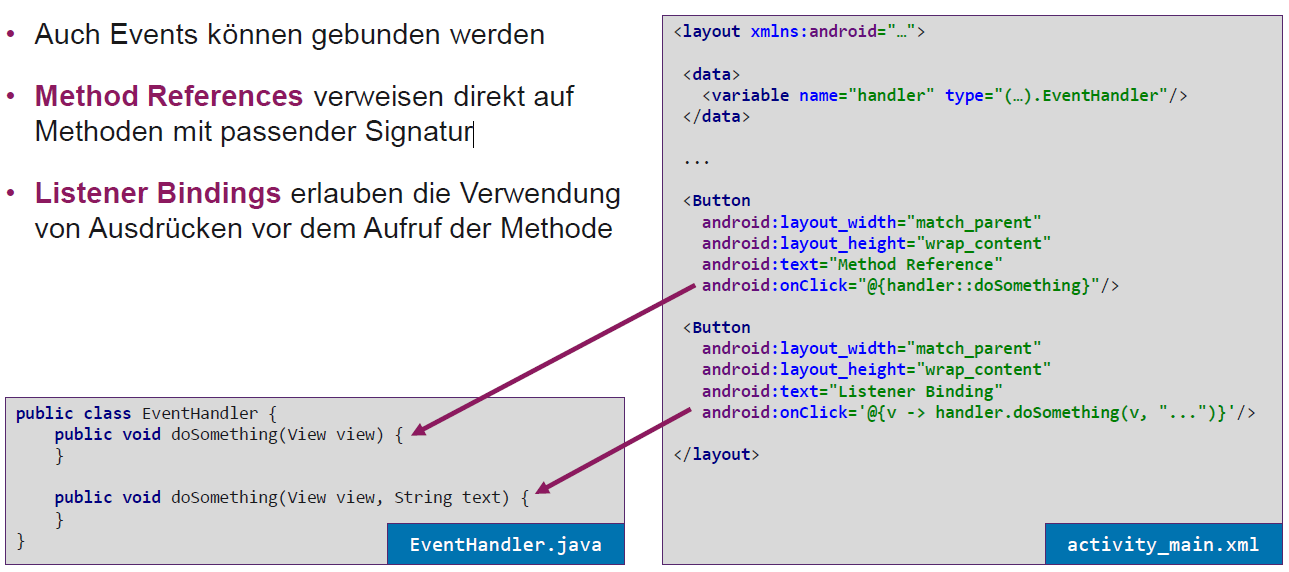
\includegraphics{data_binding_events.png}
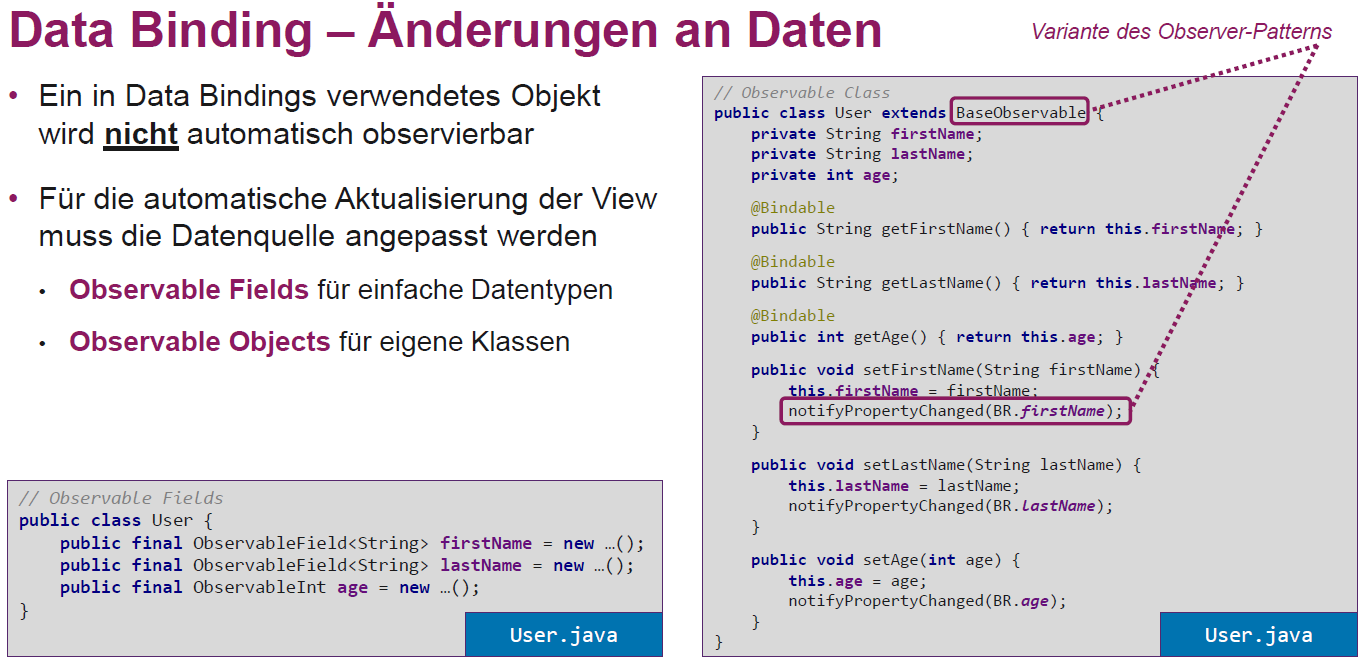
\includegraphics{data_binding_change.png}
\subsubsection{Two-Way-Bindings}
In vielen Fällen ist Two-Way nötig: z.B. Login-Checkbox in den Übungen\\
\textbf{Notation:} \textcolor{blue}{=} vor der Binding Expression

\subsection{MVVM (Model, View, View-Model)}
Durch Data Binding können schlanke, besser testbare Activites/Fragemente erstellt werden.\\
\begin{minipage}{0.6\linewidth}
    \textbf{Risiken:}
    \begin{itemize}[topsep=0pt, leftmargin=4mm]
        \setlength\itemsep{-0.3em}
        \item Model mit Android-Details verunreinigt
        \item Zu viel Logik im Layout (Expression Language)
        \item Bei Fehlern erschwertes Debugging
        \item Erhöhter Zeitbedarf für Kompilierung
        \item Gefahr für \dq unsichtbare Observer\dq
    \end{itemize}
\end{minipage}
\begin{minipage}{0.4\linewidth}
    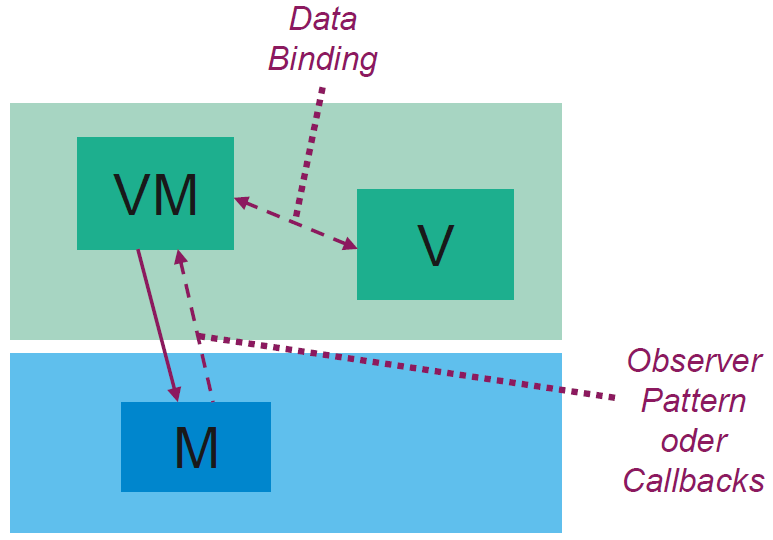
\includegraphics{mvvm.png}
\end{minipage}
\textbf{Bestandteile:}
\begin{itemize}[topsep=0pt, leftmargin=4mm]
    \setlength\itemsep{-0.3em}
    \item \textcolor{blue}{Model:} enthält Daten- und Domänenklassen (Businesslogik)
    \item \textcolor{blue}{View:} umfasst die grafische Benutzeroberfläche \& Benutzereingaben
    \item \textcolor{blue}{ViewModel:} enthält die Logik des UI und vermittelt zwischen Model und View
\end{itemize}
\textbf{Vorteile:}
\begin{itemize}[topsep=0pt, leftmargin=4mm]
    \setlength\itemsep{-0.3em}
    \item Das ViewModel ist einfach zu testen, da es keine UI-Klassen enthält
    \item Die View kümmert sich um rein visuelle Aspekte (keine Logik)
    \item Änderungen am Model haben keine Direkten Auswirkungen auf die View
\end{itemize}
\subsubsection{MVVM im Eigenbau}
\begin{lstlisting}
// UserActivity.java
public class UserActivity extends AppCompatActivity {
    private ActivityUserBinding binding;

    @Override
    protected void onCreate(Bundle savedInstanceState) {
        super.onCreate(savedInstanceState);

        User user = new User("Joel", "Schaltegger", 23);

UserViewModelFactory factory = new UseViewFactory(user);
        UserViewModel viewModel = new ViewModelProvider(
            this, factory).get(UserViewModel.class);

        binding = ActivityUserBinding.inflate(...);
        binding.setVm(viewModel);
        binding.setLifecycleOwner(this);

        setContentView(binding.getRoot());
    }
}

// UserViewModel.java
public class UserViewModel {
    private final User user;

    public final MutableLiveData<String> name = new M...<>();
    public final MutableLiveData<Integer> age = new M...<>();

    public ViewModelObservableFields(User user) {
        this.user = user;

        name.setValue(user.name);
        age.setValue(user.age);
    }

    public void incrementAge() {
        int newAge = age.getValue() + 1;
        age.setValue(newAge);
    }

    public void save() {
        user.name = name.getValue();
        user.age = age.getValue();
    }
}

// Factory.java
public class UserViewModelFactory implements ViewModelProvider.Factory {
    private final User user;

    public UserViewModelFactory(User user) {
        this.user = user;
    }

    @Override
    public <T extends ViewModel> T create(Class<T> class) {
        return (T) new UserViewModel(user);
    }
}
\end{lstlisting}
\subsection{ViewModel und Fragments}
\begin{itemize}[topsep=0pt, leftmargin=4mm]
    \setlength\itemsep{-0.3em}
    \item Die Interaktion zwischen Fragments kann sehr komplex werden
    \begin{itemize}[topsep=0pt, leftmargin=4mm]
        \setlength\itemsep{-0.3em}
        \item Viele Callback Interfaces
        \item Indirekte Kommunikation über Parent-Activity
    \end{itemize}
    \item View Models können helfen
    \begin{itemize}[topsep=0pt, leftmargin=4mm]
        \setlength\itemsep{-0.3em}
        \item Ein View Model pro Activity
        \item Fragments verwenden Teile des View Models
        \item Nachteil: Fragments verlieren Unabhängigkeit
    \end{itemize}
\end{itemize}